\documentclass[12pt]{article}
\usepackage{amsmath}
%\usepackage[paperwidth=21cm, paperheight=29.8cm]{geometry}
\usepackage[angle=0,scale=1,color=black,hshift=-0.3cm,vshift=15cm]{background}
\usepackage{multirow}
\usepackage{enumerate}

%\SetBgScale{1}
%\SetBgAngle{0}
%\SetBgColor{black}
%\SetBgContents{\rule{1pt}{30cm}}
%\SetBgHshift{-8.4cm}
%
%\backgroundsetup{contents={
%\begin{tabular}{c|c}
%\hspace{2cm} & \\[0.7cm]
%& {\bf Statistics for Computing ------ Lecture 1 ------ Solutions} \\[0.3cm]
%%\hline
%\hspace{2cm} & \hspace{18.5cm} \\ [28cm]
%\end{tabular}}}

\backgroundsetup{contents={
{\bf \centering Statistics for Computing ------------------------ Lecture 2 ------------------------------------------ Solutions} }}


\setlength{\voffset}{-3cm}
\setlength{\hoffset}{-3.45cm}
\setlength{\parindent}{0cm}
\setlength{\textheight}{27cm}
\setlength{\textwidth}{19.7cm}

\pagestyle{empty}



\begin{document}

\framebox[1.02\textwidth]{
\begin{minipage}[t]{0.98\textwidth}
\begin{minipage}[t]{0.47\textwidth}
\subsection*{Question 1}
Rearrange data.\\(needed for $Q_2$ and useful for histogram)\\[0.3cm]
\begin{tabular}{|cccccccccc|}
\multicolumn{1}{c}{\emph{1}} & \emph{2} & \emph{3} & \emph{4} & \emph{5} & \emph{6} & \emph{7} & \emph{8} & \emph{9} & \multicolumn{1}{c}{\emph{10}} \\
\hline
&&&&&&&&&\\[-0.4cm]
0 & 1 & 1 & 2 & 2 & 3 & 4 & 4 & 5 & 8 \\
\hline
\end{tabular}
\begin{enumerate}[a)]
\item $n = 10$, i.e., 10 numbers.
\item $\bar x = \frac{\sum x_i}{n} = \frac{30}{10} = 3.$
\item Population mean symbol: $\mu$. Value: unknown.
\item Position of $Q_2$ is $\frac{n+1}{2} = \frac{11}{2} = 5.5$. So $Q_2$ is the average of the numbers in positions 5 and 6.\\[0.2cm]
    $\Rightarrow$ $Q_2 = \frac{2+3}{2} = \frac{5}{2} = 2.5$.
\item $\text{width} = \frac{\max(x)-\min(x)}{\text{\# of classes}} = \frac{8-0}{3}=\frac{8}{3}=2.67.$\\[0.2cm]
    Always round up the width $\Rightarrow$ width = 3.
\end{enumerate}
\end{minipage}\hspace{0.055\textwidth}
\begin{minipage}[t]{0.47\textwidth}
\begin{enumerate}
\item[]
Starting at 0 $\Rightarrow$ 0 - 3, 3 - 6, 6 - 9. \\[0.2cm]
Classes: 0 - 2.9, 3 - 5.9, 6 - 8.9.\\[0.2cm]
\begin{tabular}{|c|r|r|}
\hline
&&\\[-0.4cm]
Class      & Freq. & R. Freq. \\
&&\\[-0.5cm]
\hline
&&\\[-0.4cm]
0 - 2.9   &   5     & $\tfrac{5}{10} = 0.5$ \\[0.2cm]
3 - 5.9   &   4     & $\tfrac{4}{10} = 0.4$ \\[0.2cm]
6 - 8.9   &   1     & $\tfrac{1}{10} = 0.1$ \\[0.2cm]
\hline
&&\\[-0.4cm]
\multicolumn{1}{|r|}{Total:} & $n = 10$ & $\tfrac{10}{10} = 1.0$ \\[0.1cm]
\hline
\end{tabular}
\item[f)]
\begin{tabular}{c}
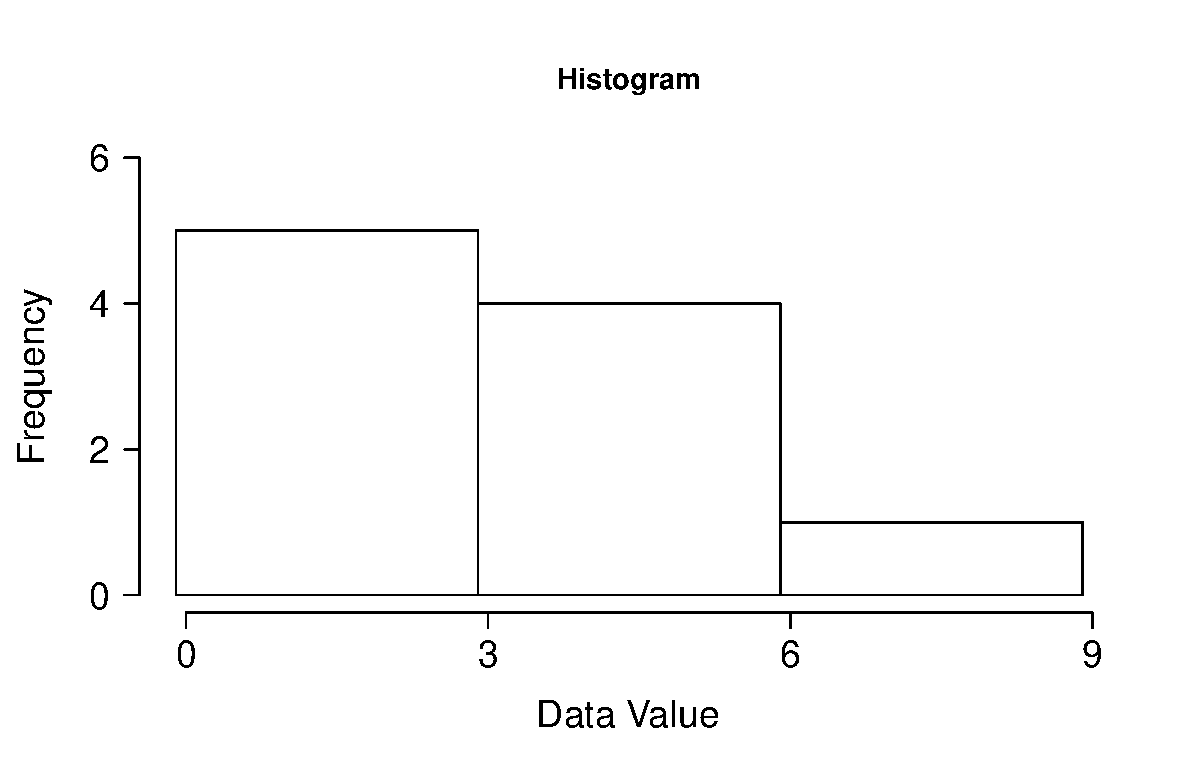
\includegraphics[width=0.9\textwidth, trim = 0.0cm 0.0cm 0.3cm 1.5cm, clip]{Hist}
\end{tabular}
\end{enumerate}
\end{minipage}
\end{minipage}}\vspace{0.03\textwidth}

\framebox[0.5\textwidth]{
\begin{minipage}[t]{0.46\textwidth}
\begin{minipage}[t]{0.35\textwidth}
\subsection*{Question 2}
Rearranged data:\\[0.2cm]
\begin{footnotesize}
\begin{tabular}{|c|cc|}
\cline{1-3}
&&\\[-0.3cm]
  & $x_i$ & $x_i^2$ \\[0.1cm]
\cline{1-3}
&&\\[-0.3cm]
1  & 0.1  &   0.01 \\
2  & 0.2  &   0.04 \\
3  & 0.2  &   0.04 \\
4  & 0.4  &   0.16 \\
5  & 0.7  &   0.49 \\
6  & 0.7  &   0.49 \\
7  & 0.9  &   0.81 \\
8  & 1.0  &   1.00 \\
9  & 1.0  &   1.00 \\
10 & 1.4  &   1.96 \\
11 & 1.5  &   2.25 \\
12 & 1.6  &   2.56 \\
13 & 2.2  &   4.84 \\
14 & 2.3  &   5.29 \\
15 & 3.0  &   9.00 \\
16 & 3.0  &   9.00 \\
17 & 3.3  &  10.89 \\
18 & 3.4  &  11.56 \\
19 & 4.2  &  17.64 \\
20 & 5.4  &  29.16 \\
21 & 5.6  &  31.36 \\
22 & 5.7  &  32.49 \\
23 & 6.1  &  37.21 \\
24 & 12.9 & 166.41  \\
25 & 14.3 & 204.49  \\
\cline{1-3}
&& \\[-0.3cm]
$\sum$ & 81.1 & 580.15 \\[0.1cm]
\cline{1-3}
\end{tabular}
\end{footnotesize}
\end{minipage}\hspace{0.055\textwidth}
\begin{minipage}[t]{0.5\textwidth}
\vspace{0.2cm}
\begin{enumerate}[a)]
\item \qquad\\[-1.55cm]
\begin{align*}
\bar x = \frac{\sum x_i}{n} &= \frac{81.1}{25}\\[0.2cm]
& = 3.244.
\end{align*}
\item \qquad\\[-1.55cm]
\begin{align*}
s^2 &= \frac{\sum x_i^2 - n\,{\bar x}^2}{n-1} \\[0.2cm]
&= \frac{580.15 - 25 \, (3.244^2)}{25-1} \\[0.2cm]
&= \frac{580.15 - 25 \, (10.524)}{24} \\[0.2cm]
&= \frac{317.05}{24} = 13.21 \, \text{hours$^2$}.\\[0.7cm]
s &= \sqrt{13.21} = 3.63 \, \text{hours}.
\end{align*}
\item The population standard deviation is $\sigma$. Its value is unknown but we estimate it with $s = 3.63$.
\item $\mu$ is the population mean (unknown).
\item This is numeric data $\Rightarrow$ no $\hat p$ here.
\end{enumerate}
\end{minipage}
\end{minipage}}\hspace{0.015\textwidth}
\framebox[0.5\textwidth]{
\begin{minipage}[t]{0.46\textwidth}
\subsection*{Question 3}
Same data as Question 2.
\begin{enumerate}[a)]
\item $n = 25$.
\item
\begin{tabular}{c|c|c}
 & {\bf Position} & {\bf Value} \\[0.1cm]
$Q_1$ & $\tfrac{n+1}{4} = \tfrac{26}{4} = 6.5$ & $\tfrac{0.7+0.9}{2} = {\bf0.8}$\\[0.3cm]
$Q_2$ & $\tfrac{n+1}{4}\times2 = 6.5(2) = 13$ & ${\bf2.2}$\\[0.3cm]
$Q_3$ & $\tfrac{n+1}{4}\times3 = 6.5(3) = 19.5$ & $\tfrac{4.2+5.4}{2} = {\bf4.8}$\\
\multicolumn{3}{c}{}\\
\end{tabular}
\item $IQR = Q_3 - Q_1 = 4.8-0.8 = 4$.
\item $\bar x = 3.244$ and $Q_2 = 2.2$.\\[0.4cm]
Since $\bar x > Q_2$ the data is skewed to the right.\\[0.4cm]
We saw this from the histogram in Question 5 of Lecture 1 also.
\end{enumerate}
\end{minipage}}\vspace{0.03\textwidth}



\framebox[1.02\textwidth]{
\begin{minipage}[t]{0.98\textwidth}
\begin{minipage}[t]{0.47\textwidth}
\subsection*{Question 4}
\begin{enumerate}[a)]
\item Type 1: $\bar x_1 = \frac{17.1}{11} =1.55.$\\[0.2cm]
Type 2: $\bar x_2 = \frac{64}{14} =4.57.$
\item $n_1 = 11$ and $n_2 = 14$.
\item Type 1\\[0.2cm]
\begin{tabular}{c|c|c}
 & {\bf Position} & {\bf Value} \\[0.1cm]
$Q_1$ & $\tfrac{n+1}{4} = \tfrac{12}{4} = 3$ & ${\bf0.2}$\\[0.3cm]
$Q_2$ & $\tfrac{n+1}{4}\times2 = 3(2) = 6$ & ${\bf0.9}$\\[0.3cm]
$Q_3$ & $\tfrac{n+1}{4}\times3 = 3(3) = 9$ & ${\bf2.3}$\\
\multicolumn{3}{c}{}\\[0.2cm]
\end{tabular}

$IQR = Q_3 - Q_1 = 2.3 - 0.2 = 2.1.$\\[0.2cm]
$LF = Q_1 - 1.5 \,IQR = 0.2-1.5(2.1)=-2.95.$\\
$UF = Q_3 + 1.5 \,IQR = 2.3+1.5(2.1)=5.45.$\\[0.1cm]
$\Rightarrow$ 5.6 is an outlier.\\[0.2cm]
Smallest non-outlier: 0.1.\\[0.1cm]
Largest non-outlier: 4.2.
\end{enumerate}
\end{minipage}\hspace{0.055\textwidth}
\begin{minipage}[t]{0.47\textwidth}
\vspace{3.1cm}
Type 2\\[0.2cm]
\begin{tabular}{c|c|c}
 & {\bf Position} & {\bf Value} \\[0.1cm]
$Q_1$ & $\tfrac{n+1}{4} = \tfrac{15}{4} = 3.75$ & $\tfrac{1.4+1.6}{2} = {\bf1.5}$\\[0.3cm]
$Q_2$ & $\tfrac{n+1}{4}\times2 = 3.75(2) = 7.5$ & $\tfrac{3.0+3.3}{2} = {\bf3.15}$\\[0.3cm]
$Q_3$ & $\tfrac{n+1}{4}\times3 = 3.75(3) = 11.25$ & $\tfrac{5.7+6.1}{2} = {\bf5.9}$\\
\multicolumn{3}{c}{}\\[0.2cm]
\end{tabular}

$IQR = Q_3 - Q_1 = 5.9 - 1.5 = 4.4.$\\[0.2cm]
$LF = Q_1 - 1.5 \,IQR = 1.5-1.5(4.4)=-5.1.$\\
$UF = Q_3 + 1.5 \,IQR = 5.9+1.5(4.4)=12.5.$\\[0.1cm]
$\Rightarrow$ 12.9 and 14.3 are outliers.\\[0.2cm]
Smallest non-outlier: 0.7.\\[0.1cm]
Largest non-outlier: 6.1.
\end{minipage}\vspace{0.03\textwidth}
\begin{minipage}[t]{1\textwidth}
\begin{center}
\begin{tabular}{c}
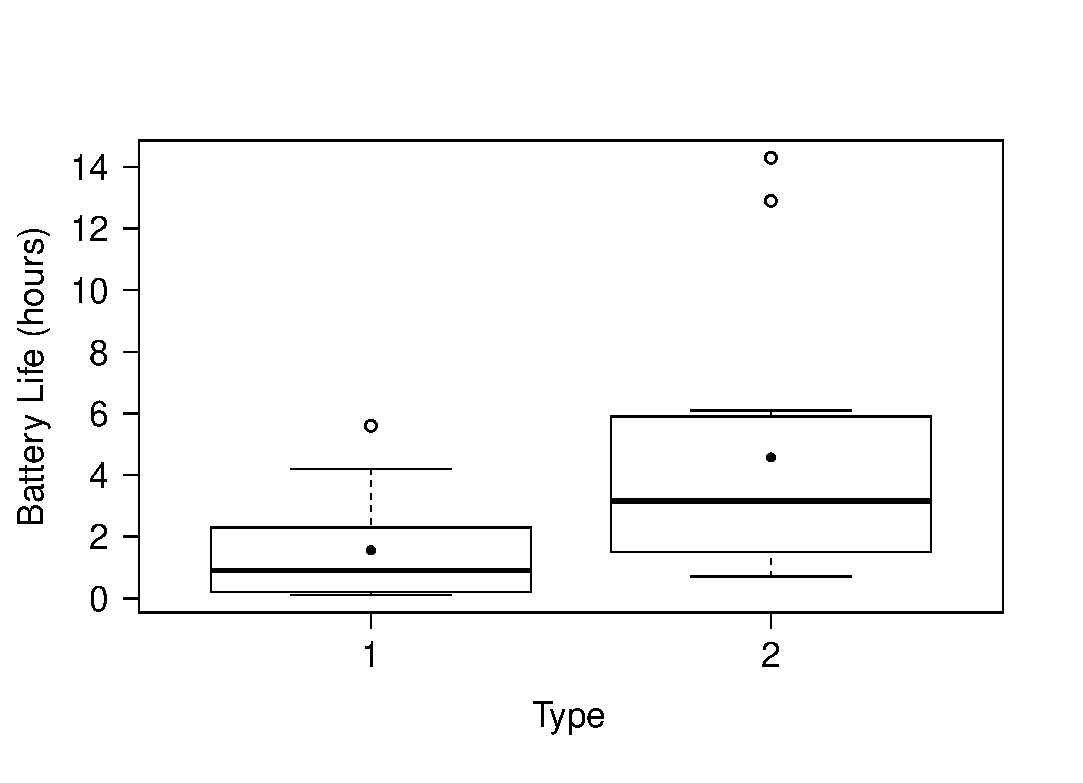
\includegraphics[width=0.7\textwidth, trim = 0.0cm 0.5cm 0.3cm 1.5cm, clip]{Boxplots}\\
\end{tabular}
\end{center}
\begin{enumerate}
\item[]
Laptops of Type 2 clearly have a greater battery life.
\item[d)] Group 1 outlier: 5.6. \quad Group 2 outliers: 12.9 and 14.3.
\item[e)] Both are skewed to the right. In both cases $\bar x > Q_2$ and also there are outliers in the right tail.
\end{enumerate}
\end{minipage}

\end{minipage}}\vspace{0.03\textwidth}


\end{document} 